

\begin{figure}[H]
	\centering			
	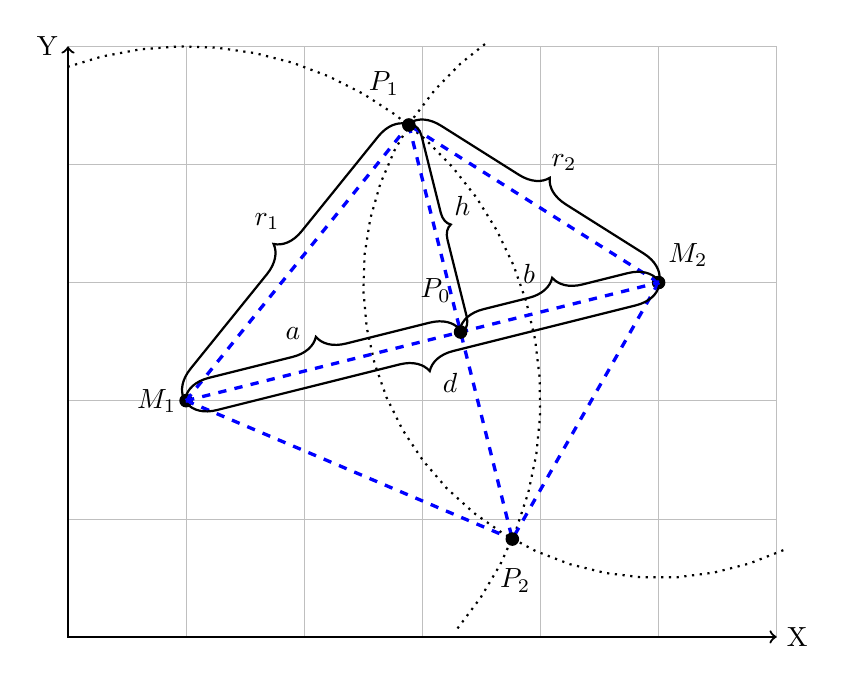
\begin{tikzpicture}[scale=1.5, domain=0:4]
		% grid
      	\draw[very thin,color=lightgray] (0,0) grid (6,5);
      	\draw [<->,thick] (0,5) node (yaxis) [left] {Y} |- (6,0) node (xaxis) [right] {X};

		% Definitions
    	\pgfmathsetlengthmacro{\ra}{3cm}
    	\pgfmathsetlengthmacro{\xa}{1cm}
    	\pgfmathsetlengthmacro{\ya}{2cm}
    
    	\pgfmathsetlengthmacro{\rb}{2.5cm}
    	\pgfmathsetlengthmacro{\xb}{5cm}
    	\pgfmathsetlengthmacro{\yb}{3cm}
	
		% The middlepoints
  		\coordinate (CA) at (\xa,\ya);
  		\coordinate (CB) at (\xb,\yb);
  
  		% The point
  		\draw[fill,color=black] (CA) circle (1.5pt) node[left, color=black] {$M_1$};
  		\draw[fill,color=black] (CB) circle (1.5pt) node[right, yshift=10pt, color=black] {$M_2$};
  
  		% The circle
  		%\draw[dashed,color=black] (CA) circle (\ra);
		%\draw[dashed,color=black] (CB) circle (\rb);
  
		\draw [dotted,thick,domain=-40:110] plot ({1+3*cos(\x)}, {2+3*sin(\x)});
		\draw [dotted,thick,domain=295:125] plot ({5+2.5*cos(\x)}, {3+2.5*sin(\x)});
	
		\coordinate (PA) at (2.885365678957660, 4.333537284169362);
    	\coordinate (PB) at (3.761693144571752, 0.828227421712991);
		\coordinate (PO) at (3.323529411764706, 2.580882352941176);
		
		\draw[very thick,color=blue,dashed] (CA) -- (CB);
      	\draw[very thick,color=blue,dashed] (PA) -- (PB);
      	\draw[very thick,color=blue,dashed] (CA) -- (PA);
      	\draw[very thick,color=blue,dashed] (CA) -- (PB);
      	\draw[very thick,color=blue,dashed] (CB) -- (PA);
      	\draw[very thick,color=blue,dashed] (CB) -- (PB);
      
      	\draw[thick,decorate,decoration={brace,amplitude=5pt,mirror,raise=1pt}] (PO) -- (PA) node[midway,xshift=10pt,yshift=8pt] {$h$};
	
\draw[thick,decorate,decoration={brace,amplitude=10pt,mirror,raise=1pt}] (CA) -- (CB) node[midway,xshift=10pt,yshift=-15pt] {$d$};
      \draw[thick,decorate,decoration={brace,amplitude=10pt,raise=1pt}] (CA) -- (PO) node[midway,xshift=-11pt,yshift=12pt] {$a$};
      \draw[thick,decorate,decoration={brace,amplitude=10pt,raise=1pt}] (PO) -- (CB) node[midway,xshift=-11pt,yshift=12pt] {$b$};	
      
      \draw[thick,decorate,decoration={brace,amplitude=10pt,raise=1pt}] (CA) -- (PA) node[midway,xshift=-11pt,yshift=15pt] {$r_1$};	
      \draw[thick,decorate,decoration={brace,amplitude=10pt,raise=1pt}] (PA) -- (CB) node[midway,xshift=+11pt,yshift=15pt] {$r_2$};	
      
      \draw[fill,color=black] (PA) circle (1.5pt) node[left, yshift=15pt, color=black] {$P_1$};
      \draw[fill,color=black] (PB) circle (1.5pt) node[left, xshift=10pt, yshift=-15pt, color=black] {$P_2$};	
      \draw[fill,color=black] (PO) circle (1.5pt) node[left, yshift=15pt, color=black] {$P_0$};
	
	\end{tikzpicture}
	\caption{Snijpunten van twee cirkels}
  	\label{fig:snijpunten}
\end{figure}

\begin{figure}[hbtp]
  \centering
  \resizebox {\textwidth} {!} {
    \begin{tikzpicture}[scale=1.5]
      % grid
      \draw[very thin,color=lightgray] (0,0) grid (7,7);
      \draw [<->,thick] (0,7) node (yaxis) [left] {Y} |- (7,0) node (xaxis) [right] {X};
      
      \circle[1,2,1.5,1]
      \circle[2,4.5,2,1]    
      \circle[3,5.5,3,1]
      \circle[4,5,5.5,1]
      
    \end{tikzpicture}
  }
  \label{fig:voorbeeld_opgave}
  \caption{Een voorbeeld opgave}
\end{figure}

\begin{figure}[hbpt]
  \centering
    \begin{tikzpicture}[scale=2]
      % grid
      \draw[very thin,color=lightgray] (0,0) grid (7,7);
      \draw [<->,thick] (0,7) node (yaxis) [left] {Y} |- (7,0) node (xaxis) [right] {X};
      
      \circle[1,2,1.5,1]
      \circle[2,4.5,2,1]    
      \circle[3,5.5,3,1]
      \circle[4,5,5.5,1]
      

      \draw[thick,color=blue,arrows={Triangle[scale=1]-Triangle[scale=1]},shorten >=9pt,shorten <=9pt] (C1) -- (C2);
      \draw[thick,color=blue,arrows={Triangle[scale=1]-Triangle[scale=1]},shorten >=9pt,shorten <=9pt] (C1) -- (C3);
      \draw[thick,color=blue,arrows={Triangle[scale=1]-Triangle[scale=1]},shorten >=9pt,shorten <=9pt] (C1) -- (C4);
      \draw[thick,color=blue,arrows={Triangle[scale=1]-Triangle[scale=1]},shorten >=9pt,shorten <=9pt] (C2) -- (C3);
      \draw[thick,color=blue,arrows={Triangle[scale=1]-Triangle[scale=1]},shorten >=9pt,shorten <=9pt] (C2) -- (C4);
      \draw[thick,color=blue,arrows={Triangle[scale=1]-Triangle[scale=1]},shorten >=9pt,shorten <=9pt] (C3) -- (C4);

      
    \end{tikzpicture}
  \label{fig:voorbeeld_1}
  \caption{Nagekeken cirkels bij algoritme 1}
\end{figure}
\begin{figure}[H]
  \centering
  \resizebox {\textwidth} {!} {
    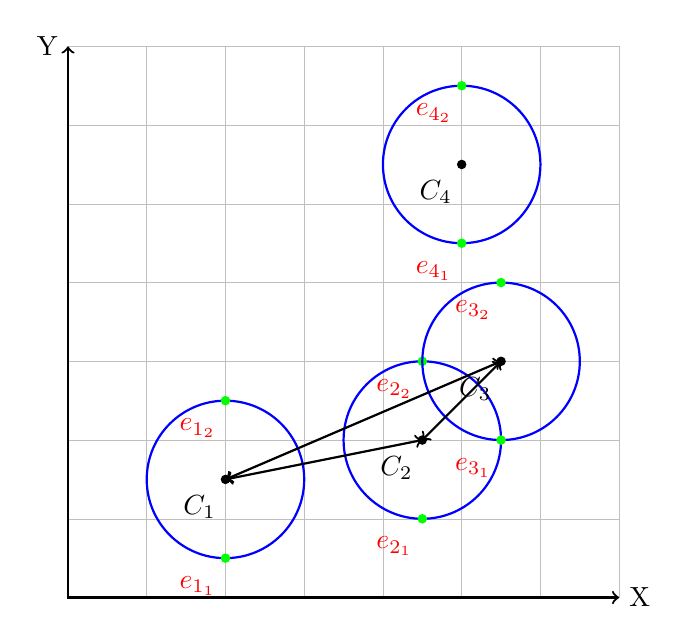
\begin{tikzpicture}[scale=1]
      % grid
      \draw[very thin,color=lightgray] (0,0) grid (7,7);
      \draw [<->,thick] (0,7) node (yaxis) [left] {Y} |- (7,0) node (xaxis) [right] {X};
      
      % Index, x, y, r
      \def\circle[#1,#2,#3,#4] {
    	% The middlepoint
    	\coordinate (C#1) at (#2,#3);
    	
    	
    	% The point
        \draw[fill,color=black] (C#1) circle (1.5pt) node[left, yshift=-10pt, color=black] {$C_#1$};
        
        % The circle
        \draw[thick,color=blue] (C#1) circle (#4);		
        
        % The eventpoints
        \coordinate (E#1_1) at (#2,#3-#4);
        \coordinate (E#1_2) at (#2,#3+#4);
    	
        \draw[fill, color=green] (E#1_1) circle (1.5pt) node[left, yshift=-10pt, color=red] {$e_{#1_1}$};
        \draw[fill, color=green] (E#1_2) circle (1.5pt) node[left, yshift=-10pt, color=red] {$e_{#1_2}$};
      }
      
      \circle[1,2,1.5,1]
      \circle[2,4.5,2,1]    
      \circle[3,5.5,3,1]
      \circle[4,5,5.5,1]
      

      \draw[thick,<->] (C1) -- (C2);
      \draw[thick,<->] (C1) -- (C3);
      \draw[thick,<->] (C2) -- (C3);


      
    \end{tikzpicture}
  }
  \label{fig:voorbeeld_2}
  \caption{Nagekeken cirkels bij algoritme 2}
\end{figure}
\begin{figure}[hbpt]
  \centering
    \begin{tikzpicture}[scale=2]
      % grid
      \draw[very thin,color=lightgray] (0,0) grid (7,7);
      \draw [<->,thick] (0,7) node (yaxis) [left] {Y} |- (7,0) node (xaxis) [right] {X};
      
      \indexedcircle[1,2,1.5,1]
      \indexedcircle[2,4.5,2,1]    
      \indexedcircle[3,5.5,3,1]
      \indexedcircle[4,5,5.5,1]

      \draw[thick,color=blue,arrows={Triangle[scale=1]-Triangle[scale=1]},shorten >=9pt,shorten <=9pt] (C2) -- (C3);

    \end{tikzpicture}
  \label{fig:voorbeeld_23}
  \caption{Nagekeken cirkels bij algoritme 3}
\end{figure}

% \begin{figure}[H]
%   \centering
%   \includegraphics[width=1\textwidth]{illustraties/fewIntersections.png}
% \end{figure}
% \begin{figure}[H]
%   \centering
%   \includegraphics[width=1\textwidth]{illustraties/manyIntersections.png}
% \end{figure}
% \begin{figure}[H]
%   \centering
%   \includegraphics[width=1\textwidth]{illustraties/3DScatter.png}
% \end{figure}

% \begin{figure}[H]
%   \centering
%   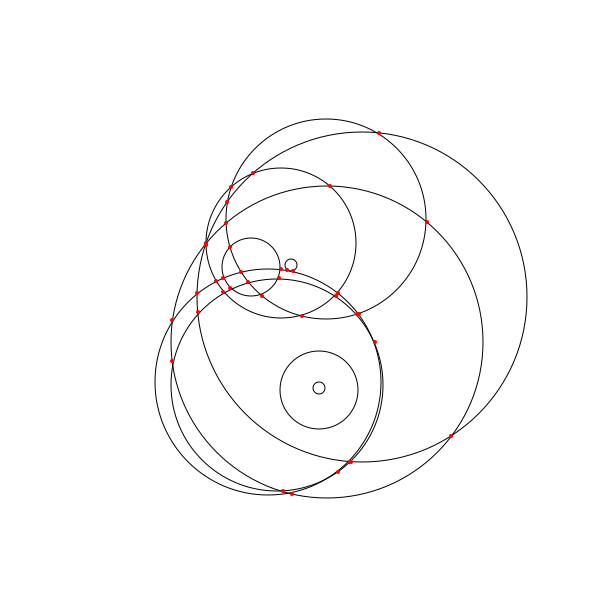
\includegraphics[width=1\textwidth]{illustraties/visuele_output.png}
% \end{figure}